\chapter{Unitarity and Sum-Rule Bounds in the Standard Model Effective Field Theory}

\begin{flushright}
\small

{\color{chapterpaperrule}\rule{\textwidth}{0.5pt}}

\textit{This chapter is based on Ref.~\cite{Bresciani:2026acy}:}\\[0.5em]
L.~C.~Bresciani, P.~Paradisi and A.~Sainaghi,\\[0pt]
``Unitarity bounds and sum rules in the SMEFT,''\\[0pt]
[\href{https://doi.org/10.48550/arXiv.2603.03423}{arXiv:2603.03423} [hep-ph]].

{\color{chapterpaperrule}\rule{\textwidth}{0.5pt}}
\end{flushright}

\section{Introduction}

\section{Conclusions}

\begin{table}[h!t!b]
\renewcommand{\arraystretch}{1.5}
    \centering
    \resizebox{\textwidth}{!}{
    \begin{tabular}{c|c|c|c|c|c|c|c|c|c}
    \toprule
    \rowcolor{hdrcolor}
    \multicolumn{2}{c|}{{\boldmath$X^3$}} & \multicolumn{2}{c|}{{\boldmath$\varphi^6$} and {\boldmath$\varphi^4D^2$}} & \multicolumn{2}{c|}{{\boldmath$   \psi^2\varphi^3$}} & \multicolumn{2}{c|}{{\boldmath$(\overline{L}L)(\overline{L}L)$}} & \multicolumn{2}{c}{{\boldmath$(\overline{L}R)(\overline{R}L)$} and {\boldmath$(\overline{L}R)(\overline{L}R)$}}\\
    \hline
    $C_G$ & $4\pi/(9g_s)$ & $C_\varphi$ & $32\pi^3/3$ & $C_{e\varphi}$ & $32\pi^2/\sqrt{3}$ & $C_{\ell\ell}$ & $2\pi$ & $C_{\ell e dq}$ & $8\pi/\sqrt{3}$ \\
    
    $C_{\widetilde G}$ & $4\pi/(9g_s)$ & $C_{\varphi\Box}$ & $8\pi/3$ & $C_{u\varphi}$ & $32\pi^2/3$ & $C_{qq}^{(1)}$ & $6\pi/5$ & $C_{quqd}^{(1)}$ & $16\pi(1+\sqrt{2})/9$\\ 
        
    $C_W$ & $2\pi/(3g)$ &$C_{\varphi D}$ & $32\pi/3$ & $C_{d\varphi}$ & $32\pi^2/3$ & $C_{qq}^{(3)}$ & $4\pi/3$ & $C_{quqd}^{(8)}$ & $4\pi(2+7\sqrt{2})/3$\\
    
    $C_{\widetilde W}$ & $2\pi/(3g)$ & & & & & $C_{\ell q}^{(1)}$ & $2\pi\sqrt{3}$ & $C_{\ell equ}^{(1)}$ & $8\pi/\sqrt{3}$ \\

    &&&&&&  $C_{\ell q}^{(3)}$ & $2\pi$ & $C_{\ell e qu}^{(3)}$ & $(2+\sqrt{2})\pi/3$   \\
    
         \midrule
         \rowcolor{hdrcolor}
         \multicolumn{2}{c|}{{\boldmath$X^2\varphi^2$}} & \multicolumn{2}{c|}{{\boldmath$\psi^2 X \varphi$}} & \multicolumn{2}{c|}{{\boldmath$\psi^2\varphi^2D$}} & \multicolumn{2}{c|}{{\boldmath$(\overline{R}R)(\overline{R}R)$}} & \multicolumn{2}{c}{{\boldmath$(\overline{L}L)(\overline{R}R)$}}\\
         \hline
         $C_{\varphi G}$ & $\pi$ & $C_{eW}$ & $4\pi\sqrt{2/3}$ & $C_{\varphi \ell}^{(1)}$ & $8\pi$ & $C_{ee}$ & $2\pi$ & $C_{\ell e}$ & $4\pi$ \\
         
         $C_{\varphi \widetilde G}$ & $\pi$ & $C_{eB}$ & $4\pi$ & $C_{\varphi \ell}^{(3)}$ & $8\pi/3$ & $C_{uu}$ & $3\pi/2$ & $C_{\ell u}$ & $4\pi$\\
         
         $C_{\varphi W}$ & $2\pi\sqrt{2/3}$ & $C_{uG}$ & $2\pi\sqrt{3}$ & $C_{\varphi e}$ & $8\pi$ & $C_{dd}$ & $3\pi/2$ & $C_{\ell d}$ & $4\pi$\\
         
         $C_{\varphi \widetilde W}$ & $2\pi\sqrt{2/3}$ & $C_{uW}$ & $4\pi\sqrt{2/3}$ & $C_{\varphi q}^{(1)}$ & $2\pi\sqrt{6}$ & $C_{eu}$ & $4\pi$ & $C_{q e}$ & $4\pi$ \\
         
        $C_{\varphi B}$ & $2\pi\sqrt{2}$ & $C_{uB}$ & $4\pi$ & $C_{\varphi q}^{(3)}$ & $8\pi/3$ & $C_{ed}$ & $4\pi$ & $C_{q u}^{(1)}$ & $2\pi\sqrt{2}$\\
        
        $C_{\varphi \widetilde B}$ & $2\pi\sqrt{2}$ & $C_{dG}$ & $2\pi\sqrt{3}$ & $C_{\varphi u}$ & $4\pi \sqrt{3}$ & $C_{ud}^{(1)}$ & $4\pi$ & $C_{q u}^{(8)}$ & $3\pi(1+1/\sqrt{2})$\\
        
        $C_{\varphi W B}$ & $4\pi$ & $C_{dW}$ & $4\pi\sqrt{2/3}$ & $C_{\varphi d}$ & $4\pi\sqrt{3}$ & $C_{ud}^{(8)}$ & $8\pi$ & $C_{qd}^{(1)}$ & $2\pi\sqrt{2}$\\
        
        $C_{\varphi \widetilde W B}$ & $4\pi$ & $C_{dB}$ & $4\pi$ & $C_{\varphi ud}$ & $8\pi$ & & & $C_{q d}^{(8)}$ & $3\pi(1+1/\sqrt{2})$ \\
        \bottomrule
    \end{tabular}
    }
    \caption{Unitarity bounds on the modulus of the baryon-number-conserving dimension-six SMEFT Wilson coefficients in the Warsaw basis \cite{Grzadkowski:2010es} (see Table \ref{tab:WarsawBasis}), obtained by marginalizing over all other SMEFT coefficients. The factors $s/\Lambda^2$ are left implicit, i.e., the reported values constrain the combination $s|C|/\Lambda^2$. Fermionic operators correspond to the single-flavor limit.}
    \label{tab:UniBounds}
\end{table}

\begin{subappendices}

\section{Conventions}
In Table \ref{tab:WarsawBasis} we report the baryon-number-conserving dimension-six operators of the SMEFT in the Warsaw basis \cite{Grzadkowski:2010es}.
%
\begin{table}[tb]
\renewcommand{\arraystretch}{1.5}
    \centering
    \resizebox{\textwidth}{!}{
    \begin{tabular}{c | c|c | c|c| c|c| c|c| c}
    \toprule
    %\toprule
    \rowcolor{hdrcolor}
    \multicolumn{2}{c|}{{\boldmath$X^3$}} & \multicolumn{2}{c|}{{\boldmath$\varphi^6$}/{\boldmath$\varphi^4D^2$}} & \multicolumn{2}{c|}{{\boldmath$\psi^2\varphi^3$}} & \multicolumn{2}{c|}{{\boldmath$(\overline{L}L)(\overline{L}L)$}} & \multicolumn{2}{c}{{\boldmath$(\overline{L}R)(\overline{R}L)$}/{\boldmath$(\overline{L}R)(\overline{L}R)$}} \\
    \hline
    $O_G$ & $f^{ABC} G_\mu^{A\nu} G_\nu^{B\rho} G_\rho^{C\mu}$ & $O_\varphi$ & $(\varphi^\dagger \varphi)^3$ & $^\ddagger O_{e\varphi}$ & $(\varphi^\dagger \varphi)(\overline{\ell}_p e_r \varphi)$ & $O_{\ell\ell}$ & $(\overline{\ell}_p \gamma_\mu \ell_r)(\overline{\ell}_s \gamma^\mu \ell_t)$ & $^\ddagger O_{\ell edq}$ & $(\overline{\ell}_p^j e_r)(\overline{d}_s q_{tj})$ \\
    
    $O_{\widetilde{G}}$ & $f^{ABC} \widetilde{G}_\mu^{A\nu} G_\nu^{B\rho} G_\rho^{C\mu}$ & $O_{\varphi\Box}$ & $(\varphi^\dagger \varphi)\Box(\varphi^\dagger \varphi)$ & $^\ddagger O_{u\varphi}$ & $(\varphi^\dagger \varphi)(\overline{q}_p u_r \widetilde{\varphi})$ & $O_{qq}^{(1)}$ & $(\overline{q}_p \gamma_\mu q_r)(\overline{q}_s \gamma^\mu q_t)$ & $^\ddagger O_{quqd}^{(1)}$ & $(\overline{q}_p^j u_r)\epsilon_{jk}(\overline{q}_s^k d_t)$ \\
    
    $O_W$ & $\epsilon^{IJK} W_\mu^{I\nu} W_\nu^{J\rho} W_\rho^{K\mu}$ & $O_{\varphi D}$ & $(\varphi^\dagger D^\mu \varphi)^* (\varphi^\dagger D_\mu \varphi)$ & $^\ddagger O_{d\varphi}$ & $(\varphi^\dagger \varphi)(\overline{q}_p d_r \varphi)$ & $O_{qq}^{(3)}$ & $(\overline{q}_p \gamma_\mu \sigma^I q_r)(\overline{q}_s \gamma^\mu \sigma^I q_t)$ & $^\ddagger O_{quqd}^{(8)}$ & $(\overline{q}_p^j T^A u_r)\epsilon_{jk}(\overline{q}_s^k T^A d_t)$ \\
    
    $O_{\widetilde{W}}$ & $\epsilon^{IJK} \widetilde{W}_\mu^{I\nu} W_\nu^{J\rho} W_\rho^{K\mu}$ & & & & & $O_{\ell q}^{(1)}$ & $(\overline{\ell}_p \gamma_\mu \ell_r)(\overline{q}_s \gamma^\mu q_t)$ & $^\ddagger O_{\ell equ}^{(1)}$ & $(\overline{\ell}_p^j e_r)\epsilon_{jk}(\overline{q}_s^k u_t)$ \\
    
    & & & & & & $O_{\ell q}^{(3)}$ & $(\overline{\ell}_p \gamma_\mu \sigma^I \ell_r)(\overline{q}_s \gamma^\mu \sigma^I q_t)$ & $^\ddagger O_{\ell equ}^{(3)}$ & $(\overline{\ell}_p^j \sigma_{\mu\nu} e_r)\epsilon_{jk}(\overline{q}_s^k \sigma^{\mu\nu} u_t)$ \\
    
    \midrule
    %\midrule
    \rowcolor{hdrcolor}
    \multicolumn{2}{c|}{{\boldmath$X^2\varphi^2$}} & \multicolumn{2}{c|}{{\boldmath$\psi^2 X \varphi$}} & \multicolumn{2}{c|}{{\boldmath$\psi^2\varphi^2D$}} & \multicolumn{2}{c|}{{\boldmath$(\overline{R}R)(\overline{R}R)$}} & \multicolumn{2}{c}{{\boldmath$(\overline{L}L)(\overline{R}R)$}} \\
    \hline
    $O_{\varphi G}$ & $(\varphi^\dagger \varphi) G_{\mu\nu}^A G^{A\mu\nu}$ & $^\ddagger O_{eW}$ & $(\overline{\ell}_p \sigma^{\mu\nu} e_r)\sigma^I \varphi W_{\mu\nu}^I$ & $O_{\varphi\ell}^{(1)}$ & $(\varphi^\dagger i\overset{\leftrightarrow}{D}{}_\mu \varphi)(\overline{\ell}_p \gamma^\mu \ell_r)$ & $O_{ee}$ & $(\overline{e}_p \gamma_\mu e_r)(\overline{e}_s \gamma^\mu e_t)$ & $O_{\ell e}$ & $(\overline{\ell}_p \gamma_\mu \ell_r)(\overline{e}_s \gamma^\mu e_t)$ \\
    
    $O_{\varphi \widetilde{G}}$ & $(\varphi^\dagger \varphi) \widetilde{G}_{\mu\nu}^A G^{A\mu\nu}$ & $^\ddagger O_{eB}$ & $(\overline{\ell}_p \sigma^{\mu\nu} e_r)\varphi B_{\mu\nu}$ & $O_{\varphi\ell}^{(3)}$ & $(\varphi^\dagger i\overset{\leftrightarrow}{D}{}_\mu^I \varphi)(\overline{\ell}_p \sigma^I \gamma^\mu \ell_r)$ & $O_{uu}$ & $(\overline{u}_p \gamma_\mu u_r)(\overline{u}_s \gamma^\mu u_t)$ & $O_{\ell u}$ & $(\overline{\ell}_p \gamma_\mu \ell_r)(\overline{u}_s \gamma^\mu u_t)$ \\
    
    $O_{\varphi W}$ & $(\varphi^\dagger \varphi) W_{\mu\nu}^I W^{I\mu\nu}$ & $^\ddagger O_{uG}$ & $(\overline{q}_p \sigma^{\mu\nu} T^A u_r)\widetilde{\varphi} G_{\mu\nu}^A$ & $O_{\varphi e}$ & $(\varphi^\dagger i\overset{\leftrightarrow}{D}{}_\mu \varphi)(\overline{e}_p \gamma^\mu e_r)$ & $O_{dd}$ & $(\overline{d}_p \gamma_\mu d_r)(\overline{d}_s \gamma^\mu d_t)$ & $O_{\ell d}$ & $(\overline{\ell}_p \gamma_\mu \ell_r)(\overline{d}_s \gamma^\mu d_t)$ \\
    
    $O_{\varphi \widetilde{W}}$ & $(\varphi^\dagger \varphi) \widetilde{W}_{\mu\nu}^I W^{I\mu\nu}$ & $^\ddagger O_{uW}$ & $(\overline{q}_p \sigma^{\mu\nu} u_r)\sigma^I \widetilde{\varphi} W_{\mu\nu}^I$ & $O_{\varphi q}^{(1)}$ & $(\varphi^\dagger i\overset{\leftrightarrow}{D}{}_\mu \varphi)(\overline{q}_p \gamma^\mu q_r)$ & $O_{eu}$ & $(\overline{e}_p \gamma_\mu e_r)(\overline{u}_s \gamma^\mu u_t)$ & $O_{qe}$ & $(\overline{q}_p \gamma_\mu q_r)(\overline{e}_s \gamma^\mu e_t)$ \\
    
    $O_{\varphi B}$ & $(\varphi^\dagger \varphi) B_{\mu\nu} B^{\mu\nu}$ & $^\ddagger O_{uB}$ & $(\overline{q}_p \sigma^{\mu\nu} u_r)\widetilde{\varphi} B_{\mu\nu}$ & $O_{\varphi q}^{(3)}$ & $(\varphi^\dagger i\overset{\leftrightarrow}{D}{}_\mu^I \varphi)(\overline{q}_p \sigma^I \gamma^\mu q_r)$ & $O_{ed}$ & $(\overline{e}_p \gamma_\mu e_r)(\overline{d}_s \gamma^\mu d_t)$ & $O_{qu}^{(1)}$ & $(\overline{q}_p \gamma_\mu q_r)(\overline{u}_s \gamma^\mu u_t)$ \\
    
    $O_{\varphi \widetilde{B}}$ & $(\varphi^\dagger \varphi) \widetilde{B}_{\mu\nu} B^{\mu\nu}$ & $^\ddagger O_{dG}$ & $(\overline{q}_p \sigma^{\mu\nu} T^A d_r)\varphi G_{\mu\nu}^A$ & $O_{\varphi u}$ & $(\varphi^\dagger i\overset{\leftrightarrow}{D}{}_\mu \varphi)(\overline{u}_p \gamma^\mu u_r)$ & $O_{ud}^{(1)}$ & $(\overline{u}_p \gamma_\mu u_r)(\overline{d}_s \gamma^\mu d_t)$ & $O_{qu}^{(8)}$ & $(\overline{q}_p \gamma_\mu T^A q_r)(\overline{u}_s \gamma^\mu T^A u_t)$ \\
    
    $O_{\varphi WB}$ & $(\varphi^\dagger \sigma^I \varphi) W_{\mu\nu}^I B^{\mu\nu}$ & $^\ddagger O_{dW}$ & $(\overline{q}_p \sigma^{\mu\nu} d_r)\sigma^I \varphi W_{\mu\nu}^I$ & $O_{\varphi d}$ & $(\varphi^\dagger i\overset{\leftrightarrow}{D}{}_\mu \varphi)(\overline{d}_p \gamma^\mu d_r)$ & $O_{ud}^{(8)}$ & $(\overline{u}_p \gamma_\mu T^A u_r)(\overline{d}_s \gamma^\mu T^A d_t)$ & $O_{qd}^{(1)}$ & $(\overline{q}_p \gamma_\mu q_r)(\overline{d}_s \gamma^\mu d_t)$ \\
    
    $O_{\varphi \widetilde{W}B}$ & $(\varphi^\dagger \sigma^I \varphi) \widetilde{W}_{\mu\nu}^I B^{\mu\nu}$ & $^\ddagger O_{dB}$ & $(\overline{q}_p \sigma^{\mu\nu} d_r)\varphi B_{\mu\nu}$ & $^\ddagger O_{\varphi ud}$ & $(\widetilde{\varphi}^\dagger i D_\mu \varphi)(\overline{u}_p \gamma^\mu d_r)$ & & & $O_{qd}^{(8)}$ & $(\overline{q}_p \gamma_\mu T^A q_r)(\overline{d}_s \gamma^\mu T^A d_t)$ \\
    \bottomrule
    %\bottomrule
    \end{tabular}
    }
    \caption{Dimension-six operators of the SMEFT in the Warsaw basis~\cite{Grzadkowski:2010es} that conserve baryon number. Non-Hermitian operators are denoted with $^\ddagger O$ and the corresponding Hermitian conjugates must be included in the Lagrangian.}
    \label{tab:WarsawBasis}
\end{table}

The relevant conventions are as follows: $\widetilde \varphi^j = \epsilon_{jk} (\varphi^k)^*$ (with $\epsilon^{12}=1$), $\varphi^\dagger \overset{\leftrightarrow}{D}{}_\mu \varphi = \varphi^\dagger D_\mu \varphi - (D_\mu \varphi)^\dagger \varphi$ and $\varphi^\dagger \overset{\leftrightarrow}{D}{}_\mu^I \varphi = \varphi^\dagger \sigma^I D_\mu \varphi - (D_\mu \varphi)^\dagger \sigma^I \varphi$, dual field-strength tensors are defined as $\widetilde X_{\mu\nu} = \frac{1}{2}\epsilon_{\mu\nu\rho\sigma}X^{\rho\sigma}$ (with $X=B,W^I,G^A$ and $\epsilon^{0123} = 1$), $\lambda^A_{\alpha\beta}$ are the Gell-Mann matrices and $\sigma^I_{jk}$ are the Pauli matrices, $T_{\alpha\beta}^A = \frac{1}{2}\lambda^A_{\alpha\beta}$ are the $SU(3)$ generators, and $\sigma_{\mu\nu} = \frac{i}{2}[\gamma_\mu,\gamma_\nu]$.
The Minkowski metric, whose signature is relevant for the spinning sum rules, is $g_{\mu\nu} = \mathrm{diag}(+1,-1,-1,-1)$.

\section{Further Details on Spinning Sum Rules\label{app: sum rules}}

In this appendix, we provide further technical details regarding the spinning sum rules discussed in Section~\ref{sec:SMEFTbounds}. 
Following Ref.~\cite{Remmen:2020uze}, we consider the amplitude $\mathcal{A}_{\alpha\beta}(s,t)$, where $s$ and $t$ are the usual Mandelstam variables associated with an elastic scattering process of
two fermions, whose quantum numbers (e.g., flavor and helicity) are collectively denoted by $\alpha$ and $\beta$.
Expanding the UV amplitude in partial waves of fixed total angular momentum, $a_{\alpha\beta}^{J}(s)$, and 
assuming vanishing boundary terms at infinity, one finds \cite{Remmen:2020uze}
%
\begin{equation}\label{eq: sum rules master equation}
    \lim_{s\rightarrow 0}\partial_s\mathcal{A}_{\overline \alpha\beta}(s,0) = -\lim_{s\rightarrow 0}\partial_s\mathcal{A}_{ \alpha\beta}(s,0) =8\int_{s_0}^\infty \dfrac{\dd s}{s^2}\left(\Im a_{\overline{\alpha}\beta}^{0}(s)-3\Im a_{\alpha\beta}^{1}(s)\right)\,,
\end{equation}
where $s_0$ is the characteristic mass-squared scale of the UV completion.\footnote{Note that our partial-wave coefficients are normalized differently from those of Ref.~\cite{Remmen:2020uze}.}
Dominance of spin-0 (spin-1) states in the UV theory implies that the left-hand side of Eq.~\eqref{eq: sum rules master equation} is positive (negative) definite for any choice of $\alpha$ and $\beta$.
This property can be exploited to derive new constraints for the flavor-dependent entries of the Wilson coefficients of four-fermion SMEFT operators, or between different $\psi^4$ operators with the same fermionic content. For completeness, we report in the following the sum-rule bounds associated with SMEFT operators in the Warsaw basis, since in Ref.~\cite{Remmen:2020uze} different conventions are used.
In particular, the combinations of Wilson coefficients reported in Table~\ref{tab:sum_rules}, when contracted with $\alpha_p \alpha_r^* \beta^*_s \beta_t$, are positive (negative) if the completion is dominated by scalars (vectors).
%
\begin{table}[h!t!b!]
\renewcommand{\arraystretch}{1.5}
    \centering
    \begin{tabular}{cc}
    \toprule
    \rowcolor{hdrcolor}
    \textbf{Operator class} & \textbf{Spinning sum rules} \\
    \midrule
    \multirow{6}{*}{\boldmath$(\overline{R}R)(\overline{R}R)$} &
    $[C_{ee}]_{prst}$ \\
    & $[C_{uu}]_{prst}$\,, \qquad $[C_{uu}]_{prst} + [C_{uu}]_{ptsr}$ \\
    & $[C_{dd}]_{prst}$\,, \qquad $[C_{dd}]_{prst} + [C_{dd}]_{ptsr}$ \\
    & $[C_{eu}]_{prst}$\,, \qquad $[C_{ed}]_{prst}$ \\
    & $[C_{ud}^{(1)}]_{prst}+\tfrac{1}{4}[C_{ud}^{(8)}]_{prst}$ \\
    & $[C_{ud}^{(1)}]_{prst}-\tfrac{1}{6}[C_{ud}^{(8)}]_{prst}$ \\
    \midrule
    \multirow{5}{*}{\boldmath$(\overline{L}L)(\overline{L}L)$} &
    $[C_{\ell\ell}]_{prst}$\,, \qquad $[C_{\ell\ell}]_{prst} + [C_{\ell\ell}]_{ptsr}$ \\
    & $[C_{qq}^{(1)}]_{prst} + [C_{qq}^{(1)}]_{ptsr} + [C_{qq}^{(3)}]_{prst} + [C_{qq}^{(3)}]_{ptsr}$ \\
    & $[C_{qq}^{(1)}]_{prst} - [C_{qq}^{(3)}]_{prst} + 2[C_{qq}^{(3)}]_{ptsr}$ \\
    & $[C_{\ell q}^{(1)}]_{prst} + [C_{\ell q}^{(3)}]_{prst}$ \\
    & $[C_{\ell q}^{(1)}]_{prst} - [C_{\ell q}^{(3)}]_{prst}$ \\
    \midrule
    \multirow{6}{*}{\boldmath$(\overline{L}L)(\overline{R}R)$} &
    $-[C_{\ell e}]_{prst}$\,, \qquad $-[C_{\ell u}]_{prst}$ \\
    & $-[C_{\ell d}]_{prst}$\,, \qquad $-[C_{qe}]_{prst}$ \\
    & $-[C_{qu}^{(1)}]_{prst} - \tfrac{1}{4}[C_{qu}^{(8)}]_{prst}$ \\
    & $-[C_{qu}^{(1)}]_{prst} + \tfrac{1}{6}[C_{qu}^{(8)}]_{prst}$ \\
    & $-[C_{qd}^{(1)}]_{prst} - \tfrac{1}{4}[C_{qd}^{(8)}]_{prst}$ \\
    & $-[C_{qd}^{(1)}]_{prst} + \tfrac{1}{6}[C_{qd}^{(8)}]_{prst}$ \\
    \bottomrule
    \end{tabular}
    \caption{Combinations of four-fermion Wilson coefficients that, when contracted with $\alpha_p \alpha_r^* \beta^*_s \beta_t$, are positive (negative) if the UV completion is dominated by scalars (vectors).}
    \label{tab:sum_rules}
\end{table}
%
As a final remark, we stress that these bounds are subject to some limitations that may lead to their violation, as already discussed in the main text.

\section{Matching of Ultraviolet Completions}

To illustrate both the diagnostic power and the limitations of the spinning sum
rules discussed in the main text and Appendix~\ref{app: sum rules}, we match a
representative set of single-field, tree-level UV completions \cite{deBlas:2017xtg}
onto the third-generation semileptonic operators $[O_{\ell q}^{(1)}]_{3333}$ and
$[O_{\ell q}^{(3)}]_{3333}$, whose unitarity and sum-rule constraints are shown in
Figure~\ref{fig:3plots} (right). The results are collected in Table~\ref{tab:models}.
%
\begin{table}[tb]
\renewcommand{\arraystretch}{1}
    \centering
    \resizebox{\textwidth}{!}{
    \begin{tabular}{ccccccc}
    %\toprule
    \toprule
    \rowcolor{hdrcolor}
    \textbf{Field}  & \textbf{Spin} & \textbf{Channel} & \boldmath$[C_{\ell q}^{(1)}]_{3333}/\Lambda^2$ & \boldmath$[C_{\ell q}^{(3)}]_{3333}/\Lambda^2$ & \textbf{Unitarity Bound} & \textbf{Plot} \\
    \midrule
    % $\omega_1$ & $(3,1)_{-\displaystyle\frac{1}{3}}$ & $0$ & $s$ & $\displaystyle\frac{|[y^{q\ell}_{\omega_1}]_{33}|^2}{4M^2_{\omega_1}}$ & $\displaystyle\frac{-|[y^{q\ell}_{\omega_1}]_{33}|^2}{4M^2_{\omega_1}}$ & $\displaystyle\frac{|[y^{q\ell}_{\omega_1}]_{33}|^2 s}{4\pi M^2_{\omega_1}}\leq 1$ & \makecell[c]{\includegraphics[scale = 0.5]{images/omega1.pdf}} \\
    % $\zeta$ & $(3,3)_{-\displaystyle\frac{1}{3}}$ & $0$ & $s$ & $3|[y^{q\ell}_{\zeta}]_{33}|^2/(4M^2_{\zeta})$ & $|[y^{q\ell}_{\zeta}]_{33}|^2/(4M^2_{\zeta})$ & $|[y^{q\ell}_{\zeta}]_{33}|^2\,s\leq 4\pi M^2_{\zeta}$ & \makecell[c]{\includegraphics[scale = 0.5]{images/zeta.pdf}} \\
    % $\mathcal{U}_2$ & $(3,1)_{\displaystyle\frac{2}{3}}$ & $1$ & $s$ & $-|[g_{\mathcal U_2}^{\ell q}]_{33}|^2/(2M^2_{\mathcal U_2})$ & $-|[g_{\mathcal U_2}^{\ell q}]_{33}|^2/(2M^2_{\mathcal U_2})$ & $|[g_{\mathcal U_2}^{\ell q}]_{33}|^2\,s\leq 4\pi M^2_{\mathcal U_2}$ & \makecell[c]{\includegraphics[scale = 0.5]{images/U2.pdf}} \\
    % $\mathcal{X}$ & $(3,3)_{\displaystyle\frac{2}{3}}$ & $1$ & $s$ & $-3|[g_{\mathcal X}]_{33}|^2/(8M^2_{\mathcal X})$ & $|[g_{\mathcal X}]_{33}|^2/(8M^2_{\mathcal X})$ & $|[g_{\mathcal X}]_{33}|^2\,s\leq \tfrac{16}{3}\pi M^2_{\mathcal X}$ & \makecell[c]{\includegraphics[scale = 0.5]{images/X.pdf}} \\
    % $\mathcal{B}$ & $(1,1)_{0}$ & $1$ & $t$ & $-[g_{\mathcal B}^\ell]_{33}[g_{\mathcal B}^q]_{33}/M^2_{\mathcal B}$ & $0$ & $|[g_{\mathcal B}^\ell]_{33}[g_{\mathcal B}^q]_{33}|\,s\leq 2\sqrt{3}\,\pi M^2_{\mathcal B}$ & \makecell[c]{\includegraphics[scale = 0.5]{images/B.pdf}} \\
    % $\mathcal{W}$ & $(1,3)_{0}$ & $1$ & $t$ & $0$ & $-[g_{\mathcal W}^\ell]_{33}[g_{\mathcal W}^q]_{33}/(4M^2_{\mathcal W})$ & $|[g_{\mathcal W}^\ell]_{33}[g_{\mathcal W}^q]_{33}|\,s\leq \tfrac{16}{3}\pi M^2_{\mathcal W}$ & \makecell[c]{\includegraphics[scale = 0.5]{images/W.pdf}} \\
    % \bottomrule
    $\omega_1\sim(3,1)_{-\frac{1}{3}}$ & $0$ & $s$ & $\displaystyle\frac{|[y^{q\ell}_{\omega_1}]_{33}|^2}{4M^2_{\omega_1}}$ & $\displaystyle\frac{-|[y^{q\ell}_{\omega_1}]_{33}|^2}{4M^2_{\omega_1}}$ & $\displaystyle\frac{|[y^{q\ell}_{\omega_1}]_{33}|^2 s}{4\pi M^2_{\omega_1}}\leq 1$ & \makecell[c]{\includegraphics[scale = 0.8,page=6]{images/UVfield.pdf}} \\
$\zeta\sim(3,3)_{-\frac{1}{3}}$ & $0$ & $s$ & $\displaystyle\frac{3|[y^{q\ell}_{\zeta}]_{33}|^2}{4M^2_{\zeta}}$ & $\displaystyle\frac{|[y^{q\ell}_{\zeta}]_{33}|^2}{4M^2_{\zeta}}$ & $\displaystyle\frac{|[y^{q\ell}_{\zeta}]_{33}|^2s}{4\pi M^2_{\zeta}}\leq 1$ & \makecell[c]{\includegraphics[scale = 0.8,page=5]{images/UVfield.pdf}} \\
$\mathcal{U}_2\sim(3,1)_{\frac{2}{3}}$ & $1$ & $s$ & $\displaystyle\frac{-|[g_{\mathcal U_2}^{\ell q}]_{33}|^2}{2M^2_{\mathcal U_2}}$ & $\displaystyle\frac{-|[g_{\mathcal U_2}^{\ell q}]_{33}|^2}{2M^2_{\mathcal U_2}}$ & $\displaystyle\frac{|[g_{\mathcal U_2}^{\ell q}]_{33}|^2s}{4\pi M^2_{\mathcal U_2}}\leq 1$ & \makecell[c]{\includegraphics[scale = 0.8,page=4]{images/UVfield.pdf}} \\
$\mathcal{X}\sim(3,3)_{\frac{2}{3}}$ & $1$ & $s$ & $\displaystyle\frac{-3|[g_{\mathcal X}]_{33}|^2}{8M^2_{\mathcal X}}$ & $\displaystyle\frac{|[g_{\mathcal X}]_{33}|^2}{8M^2_{\mathcal X}}$ & $\displaystyle\frac{3|[g_{\mathcal X}]_{33}|^2s}{16\pi M^2_{\mathcal X}}\leq 1$ & \makecell[c]{\includegraphics[scale = 0.8,page=3]{images/UVfield.pdf}} \\
$\mathcal{B}\sim(1,1)_{0}$ & $1$ & $t$ & $\displaystyle\frac{-[g_{\mathcal B}^\ell]_{33}[g_{\mathcal B}^q]_{33}}{M^2_{\mathcal B}}$ & $0$ & $\displaystyle\frac{|[g_{\mathcal B}^\ell]_{33}[g_{\mathcal B}^q]_{33}|s}{2\sqrt{3}\pi M^2_{\mathcal B}}\leq 1$ & \makecell[c]{\includegraphics[scale = 0.8,page=2]{images/UVfield.pdf}} \\
$\mathcal{W}\sim(1,3)_{0}$ & $1$ & $t$ & $0$ & $\displaystyle\frac{-[g_{\mathcal W}^\ell]_{33}[g_{\mathcal W}^q]_{33}}{4M^2_{\mathcal W}}$ & $\displaystyle\frac{3|[g_{\mathcal W}^\ell]_{33}[g_{\mathcal W}^q]_{33}|s}{16\pi M^2_{\mathcal W}}\leq 1$ & \makecell[c]{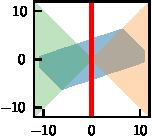
\includegraphics[scale = 0.8,page=1]{images/UVfield.pdf}} \\
\bottomrule
    \end{tabular}
    }
    \caption{Tree-level matching of single-field UV completions \cite{deBlas:2017xtg}
    onto $[O_{\ell q}^{(1)}]_{3333}$ and $[O_{\ell q}^{(3)}]_{3333}$. The penultimate
    column reports the associated perturbative unitarity bound, obtained as the most
    stringent of the constraints for $[C_{\ell q}^{(1)}]_{3333}$ and $[C_{\ell q}^{(3)}]_{3333}$ evaluated on the
    matched Wilson coefficients. The last column contains the plots in the plane $(s[C_{\ell q}^{(1)}]_{3333}/\Lambda^2, s[C_{\ell q}^{(3)}]_{3333}/\Lambda^2)$, where the blue, orange, and green regions correspond to those consistent with unitarity bounds and spin-$0$ and spin-$1$ sum-rule constraints, respectively, while the red lines indicate where each model lies: the scalar and vector leptoquarks are correctly classified by
    their spin, whereas the $t$-channel vectors evade the classification.}
    \label{tab:models}
\end{table}

The two scalar leptoquarks ($\omega_1$, $\zeta$) and the two vector leptoquarks
($\mathcal{U}_2$, $\mathcal{X}$) generate these operators through $s$-channel
exchange in the elastic $\ell q \to \ell q$ amplitude, and therefore enter the
dispersion relation of Eq.~\eqref{eq: sum rules master equation} with their physical
spin. 
Explicitly, the relevant combinations of Table~\ref{tab:sum_rules},
$[C_{\ell q}^{(1)}]_{3333} \pm [C_{\ell q}^{(3)}]_{3333}$, are both non-negative for
$\omega_1$ and $\zeta$, and both non-positive for $\mathcal{U}_2$ and $\mathcal{X}$,
so that the scalar (vector) leptoquarks are correctly placed in the scalar-
(vector-) dominated region of Figure~\ref{fig:3plots} (right).

By contrast, the color-singlet vectors $\mathcal{B} \sim (1,1)_0$ and
$\mathcal{W} \sim (1,3)_0$ couple separately to the lepton and quark currents and are exchanged in the $t$-channel. The boundary terms then no longer vanish, modifying Eq.~\eqref{eq: sum rules master equation}, and the sum-rule
classification fails: $\mathcal{W}$ yields combinations of opposite sign and thus
lies outside both the scalar- and vector-dominated regions, while $\mathcal{B}$ can
fall in the region associated with the opposite (scalar) spin, depending on the sign
of $[g_{\mathcal B}^\ell]_{33}[g_{\mathcal B}^q]_{33}$. These cases provide explicit
examples of the statement made in the main text that vector $t$-channel completions
can violate the spinning sum-rule constraints, whereas all tree-level scalar
completions satisfy them.

\section{Mathematical Tools}

\subsection{Logical Expression}\label{sec:appendix, logical expression}

The function $f(x) = a + bx - \sqrt{c^2 + dx + ex^2}$ --- assumed real on $[0,1]$ and with $a,b,c,d,e\in\mathbb{R}$ --- is such that $f(x) \ge 0$ for every $x \in [0,1]$ if and only if the system of inequalities
\begin{align}
    \Delta(a,b,c,d,e) &= 
    a \ge 0 
    \ \land \
    a+b \ge 0
    \ \land \ 
    a^2 - c^2 \ge 0
    \ \land \ 
    (a+b)^2 - c^2 -d-e \ge 0 \nonumber
    \\& \quad
    \land \
    [e - b^2 \ge 0 \ \lor\  (2ab-d)(2ab-d+2b^2-2e) \ge 0 \nonumber 
    \\& \quad
    \lor \ 4(b^2-e)(a^2-c^2)-(2ab-d)^2 \ge 0]
\end{align}
is true.

To prove this, note that,
since $g(x)=c^2 + dx + ex^2 \ge 0$ on $[0,1]$ by assumption, $f(x) \ge 0$ on $[0,1]$ is equivalent to $\ell(x) = a + bx \ge 0$ and $h(x) = \ell(x)^2 -g(x) \ge 0$ on $[0,1]$. The latter reads $h(x) = \alpha x^2 + \beta x + \gamma$, with $\alpha = b^2-e$, $\beta = 2ab-d$, and $\gamma=a^2-c^2$.
Thus, it is sufficient to prove that $p(x) = \alpha x^2+\beta x + \gamma \ge 0$ on $[0,1]$ if and only if
    \begin{equation}\label{eq:lemma}
        \gamma\ge0 \ \land \ \alpha+\beta+\gamma\ge0 \ \land \
    [\alpha\le0 \ \lor \ \beta(\beta+2\alpha)\ge0 \ \lor \ 4\alpha\gamma-\beta^2\ge0 ] \,.
    \end{equation}
Indeed, $\Delta$ is exactly Eq.~\eqref{eq:lemma} applied to $\ell$ and $h$.
The first two conditions in Eq.~\eqref{eq:lemma} are $p(0)\ge 0$ and $p(1)\ge 0$, thus they are necessary; assume them in what follows. If $\alpha \le 0$, then $p$ is concave and has its minimum on $[0,1]$ at an endpoint, so $p\ge 0$; instead, if $\alpha >0$, the vertex is at $x_\ast = -\beta/(2\alpha)$, and
\begin{equation}
    x_\ast\le0 \iff \beta\ge0 \,, \qquad x_\ast\ge1 \iff \beta+2\alpha\le0 \,,
\end{equation}
so $x_\ast \notin (0,1)$ if and only if $\beta(\beta+2\alpha)\ge 0$, in which case the minimum is again at an endpoint and $p\ge 0$. Otherwise, $x_\ast \in (0,1)$ and $\min_{[0,1]} p = p(x_\ast) = (4\alpha\gamma-\beta^2)/(4\alpha)$, which has the same sign as $4\alpha\gamma-\beta^2$. The last condition is then both necessary and sufficient. 

\subsection{Eigenvalues of Jordan--Wielandt Matrices}

Given the Hermitian Jordan--Wielandt matrix
\begin{equation}
    M=\begin{pmatrix}
        \mathbb{O}_{m\times m} & A \\ A^\dag & \mathbb{O}_{n\times n}
    \end{pmatrix}
\end{equation}
of size $m+n$,
with $A\in \mathbb{C}^{m \times n}$,
we have that its characteristic polynomial --- with the convention $p_X(x) = \det(x\mathbb{1}-X)$ --- is
\begin{equation}
    p_M(x)=x^{n-m}\,p_{AA^\dag}(x^2) = x^{m-n}\,p_{A^\dag A}(x^2) \,,
\end{equation}
which means that the eigenvalues of $M$ can be computed as the positive and negative square roots of the eigenvalues of $AA^\dag$ if $m\le n$ (of $A^\dag A$ if $m > n$), together with additional $\abs{n-m}$ vanishing eigenvalues. 
%

To prove this, consider a generic block matrix that takes the form
\begin{equation}
    \begin{pmatrix}
        P & Q \\ R & S
    \end{pmatrix}\,.
\end{equation}
If $S$ is invertible, then
\begin{equation}
    \begin{pmatrix}
        P & Q \\ R & S
    \end{pmatrix}
    \begin{pmatrix} \mathbb{1} & \mathbb{O} \\ -S^{-1}R & \mathbb{1} 
    \end{pmatrix}
    =
    \begin{pmatrix} P-QS^{-1}R & Q \\ \mathbb{O} & S 
    \end{pmatrix}\,,
\end{equation}
which implies that 
\begin{equation}
    \det\begin{pmatrix} P & Q \\ R & S \end{pmatrix}=\det(P-QS^{-1}R) \det S \,.
\end{equation}
By applying this to the matrix $x\mathbb{1}_{(m+n)\times(m+n)}-M$, we find the result above.

\end{subappendices}